\documentclass[11pt,a4paper]{article}

% ---------- Packages ----------
\usepackage[utf8]{inputenc}
\usepackage[T1]{fontenc}
\usepackage{lmodern}
\usepackage[margin=1in]{geometry}
\usepackage{graphicx}
\usepackage{float}
\usepackage{booktabs}
\usepackage{array}
\usepackage{longtable}
\usepackage{multirow}
\usepackage{xcolor}
\usepackage{amsmath, amssymb}
\usepackage{enumitem}
\usepackage{hyperref}
\usepackage{caption}
\usepackage{subcaption}
\usepackage{fancyhdr}
\usepackage{setspace}
\usepackage{tabularx}
\usepackage{tikz}
\usepackage{url}

% ---------- Formatting ----------
\hypersetup{
    colorlinks=true,
    linkcolor=blue,
    urlcolor=blue,
    citecolor=blue
}

\setlength{\parindent}{0pt}
\setlength{\parskip}{0.6em}
\onehalfspacing
\setlength{\headheight}{14pt}

\pagestyle{fancy}
\fancyhf{}
\lhead{Information Visualization Homework}
\rhead{\thepage}

% Section formatting (kept simple to avoid extra package dependencies)
%\titleformat{\section}{\large\bfseries}{\thesection.}{0.5em}{}
%\titleformat{\subsection}{\normalsize\bfseries}{\thesubsection.}{0.5em}{}

% ---------- Helper commands ----------
\newcommand{\placeholder}[1]{\textcolor{gray}{\textit{#1}}}
\newcommand{\githublink}{\url{https://github.com/your-username/your-repository}}

\begin{document}

\begin{titlepage}
    \centering
    {\Large Sabancı University \par}
    \vspace{1.2cm}
    {\LARGE \textbf{Information Visualization Homework Report} \par}
    \vspace{0.8cm}
    {\large Population Change and Socio-Economic Indicators in Türkiye (2019--2024)\par}
    \vspace{1.5cm}

    \begin{tabular}{rl}
        \textbf{Student Name:} & \placeholder{Write your name here} \\
        \textbf{Student ID:} & \placeholder{Write your ID here} \\
        \textbf{Course:} & \placeholder{Write course code/name here} \\
        \textbf{Instructor:} & \placeholder{Write instructor name here} \\
        \textbf{Submission Date:} & \placeholder{Write date here} \\
    \end{tabular}

    \vfill

    \textbf{Project Question}\\[0.4em]
    \fbox{%
        \parbox{0.9\textwidth}{%
        What relationship exists between population growth in major Turkish cities and national socio-economic indicators such as unemployment rate, GDP per capita, and inflation between 2019 and 2024?
        }
    }

    \vfill
\end{titlepage}

\tableofcontents
\newpage

% =========================================================
\section{Introduction}

This report presents the design process and implementation for a visualization homework project based on Turkish population and socio-economic data. The study focuses on the years 2019 to 2024 and investigates whether changes in the populations of selected major cities move together with national indicators such as unemployment rate, GDP per capita, and inflation.

The report combines hand-drawn sketches, design rationale, and one coded visualization. Some sections intentionally contain placeholders so that additional handwritten images, screenshots, reflections, and course-specific terminology can be inserted later.

\textbf{Main research question:}

What relationship exists between population growth in major Turkish cities and national socio-economic indicators such as unemployment rate, GDP per capita, and inflation between 2019 and 2024?

% =========================================================
\section{Dataset Description}

\subsection{Scope of the Study}

Although the original census dataset covered a broader time interval, only the years between 2019 and 2024 were used in this homework in order to align the population data with the socio-economic indicators collected for the same period.

The selected cities are:
\begin{itemize}[leftmargin=1.5em]
    \item Van
    \item Muğla
    \item Adana
    \item Ankara
    \item İstanbul
    \item İzmir
\end{itemize}

\subsection{Population Data Used}

\begin{table}[H]
\centering
\caption{Population of Selected Turkish Cities (2019--2024)}
\small
\begin{tabular}{lrrrrrr}
\toprule
\textbf{Year} & \textbf{Van} & \textbf{Muğla} & \textbf{Adana} & \textbf{Ankara} & \textbf{İstanbul} & \textbf{İzmir} \\
\midrule
2019 & 1,136,757 & 983,142 & 2,237,940 & 5,639,076 & 15,519,267 & 4,367,251 \\
2020 & 1,149,342 & 1,000,773 & 2,258,718 & 5,663,322 & 15,462,452 & 4,394,694 \\
2021 & 1,141,015 & 1,021,141 & 2,263,373 & 5,747,325 & 15,840,900 & 4,425,789 \\
2022 & 1,128,749 & 1,048,185 & 2,274,106 & 5,782,285 & 15,907,951 & 4,462,056 \\
2023 & 1,127,612 & 1,066,736 & 2,270,298 & 5,803,482 & 15,655,924 & 4,479,525 \\
2024 & 1,118,087 & 1,081,867 & 2,280,484 & 5,864,049 & 15,701,602 & 4,493,242 \\
\bottomrule
\end{tabular}
\end{table}

\subsection{Average Population Values Used in Some Sketches}

For some sketches, an average city population value was used for simplicity and readability.

\begin{table}[H]
\centering
\caption{Average Population Used in Simplified Sketches}
\begin{tabular}{lr}
\toprule
\textbf{Year} & \textbf{Average Population} \\
\midrule
2019 & 4,980,572 \\
2020 & 5,021,550 \\
2021 & 5,073,257 \\
2022 & 5,100,555 \\
2023 & 5,067,263 \\
2024 & 5,089,889 \\
\bottomrule
\end{tabular}
\end{table}

\subsection{Socio-Economic Indicators from TÜİK}

The three national indicators selected from TÜİK for the same period are unemployment rate, GDP per capita (USD), and inflation rate.

\begin{table}[H]
\centering
\caption{National Socio-Economic Indicators of Türkiye (2019--2024)}
\begin{tabular}{lrrr}
\toprule
\textbf{Year} & \textbf{Unemployment Rate} & \textbf{GDP per Capita (USD)} & \textbf{Inflation Rate} \\
\midrule
2019 & 13.7 & 9127 & 11.84 \\
2020 & 13.2 & 8555 & 14.60 \\
2021 & 12.0 & 9592 & 36.08 \\
2022 & 10.4 & 10655 & 62.93 \\
2023 & 9.4 & 13243 & 64.00 \\
2024 & 8.6 & 15325 & 44.38 \\
\bottomrule
\end{tabular}
\end{table}

% =========================================================
\section{Task 1: Hand-Drawn Exploratory Sketches}

\subsection{Task 1: Türkiye Map with City-Based Time Series}

In this task, a hand-drawn map of Türkiye was created, and the six selected cities were placed and labeled on the map. Next to each city, a small time-series line chart was drawn to show population change between 2019 and 2024.

\begin{figure}[H]
    \centering
    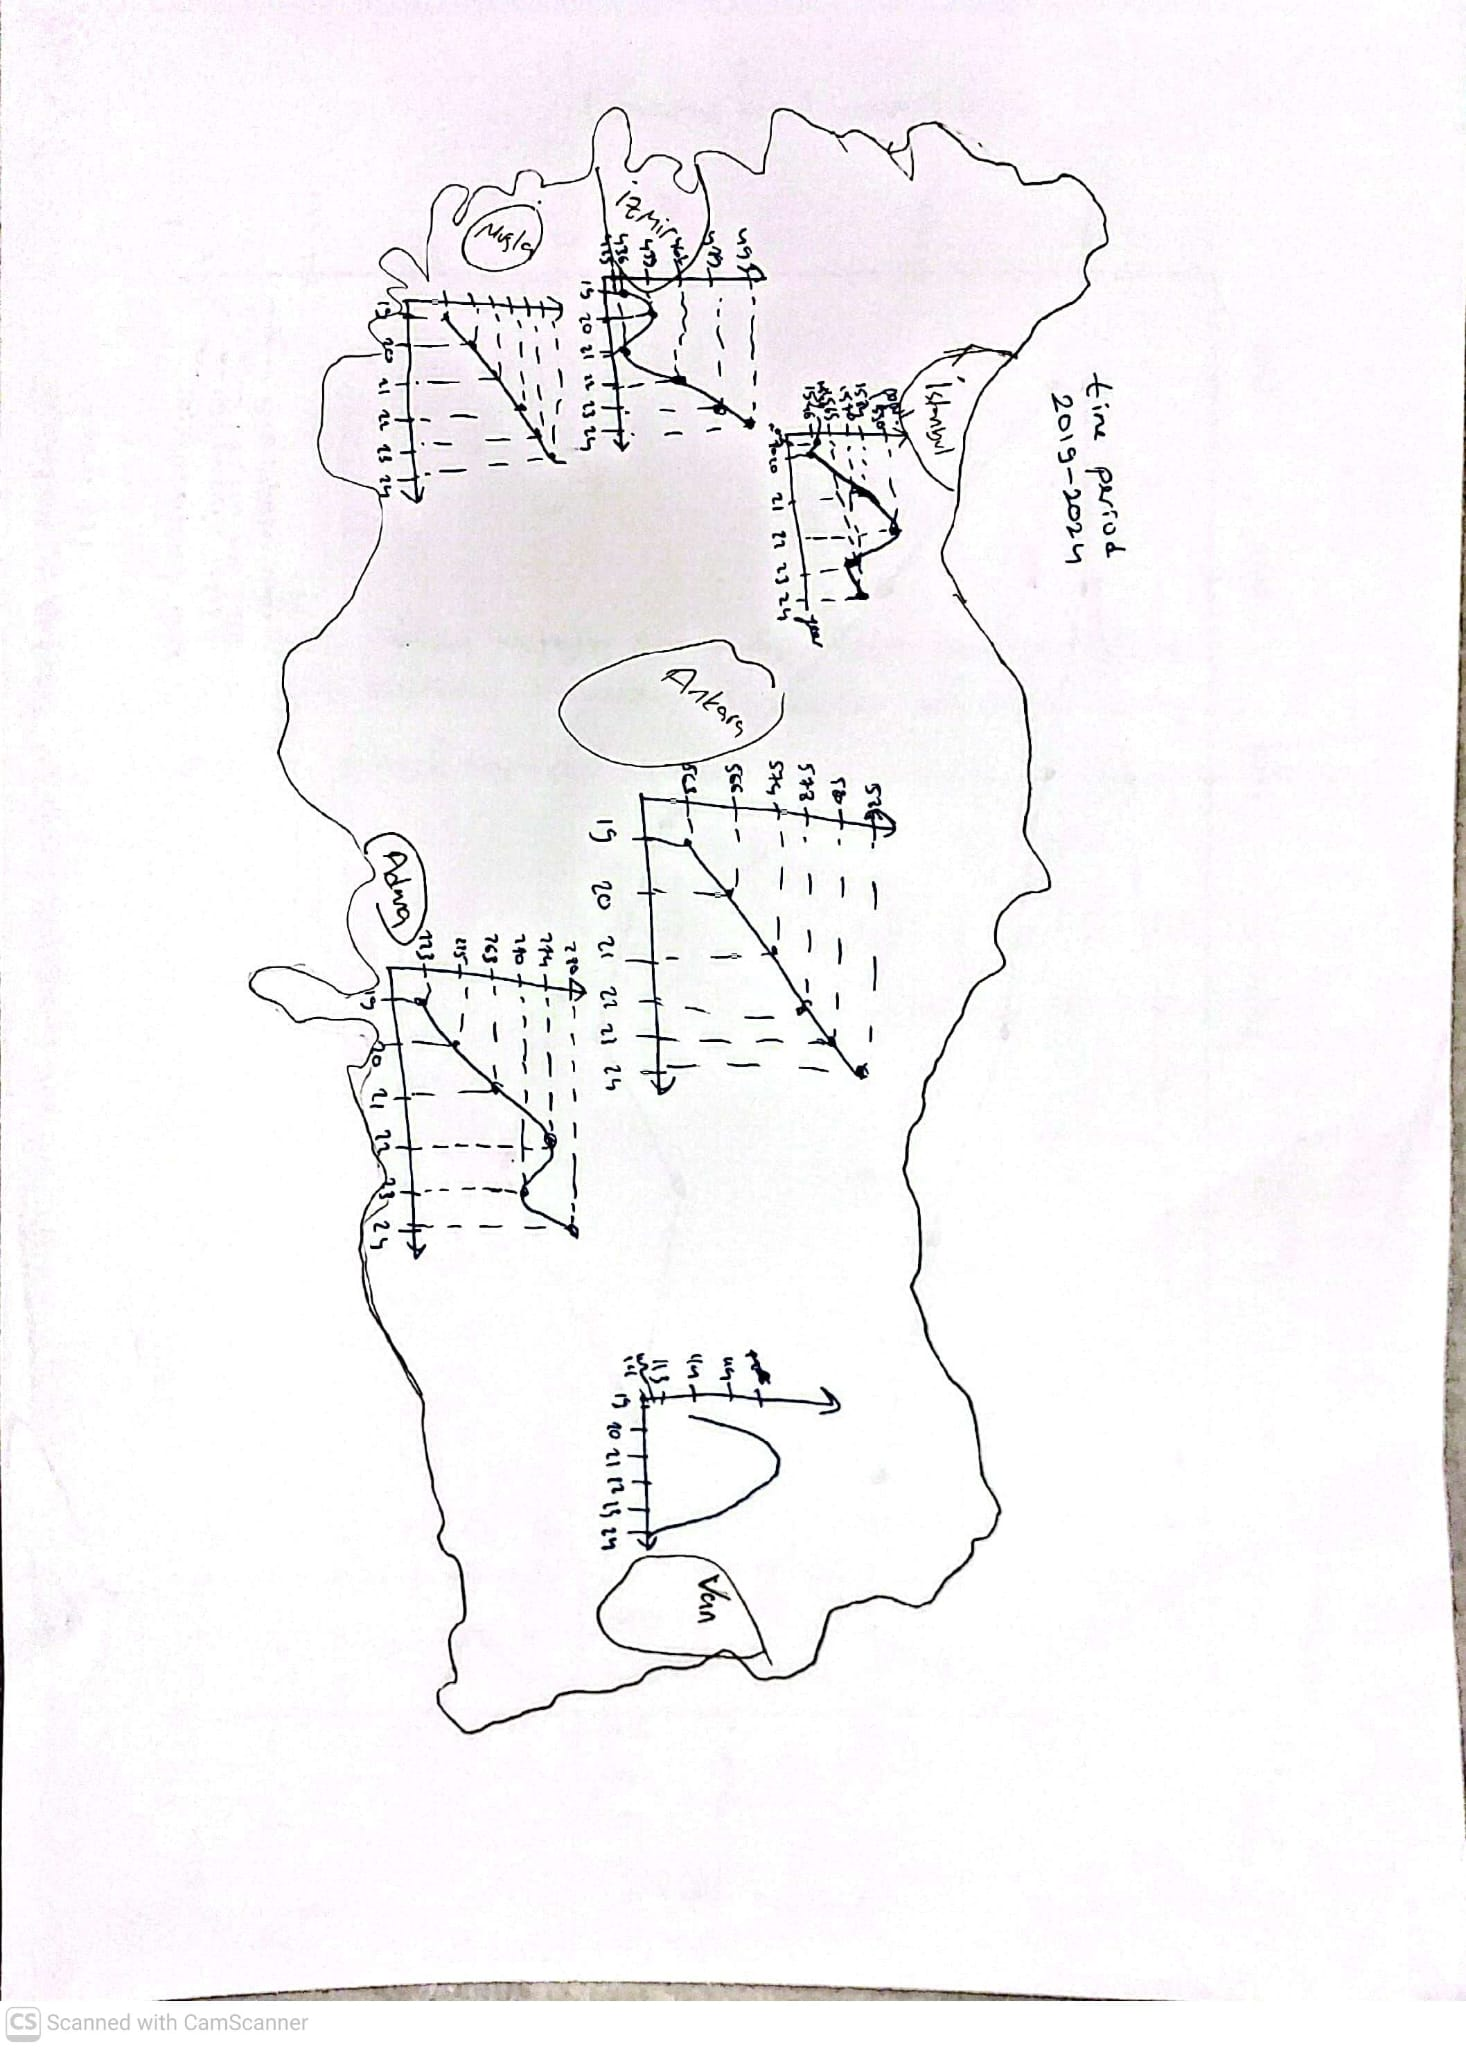
\includegraphics[width=0.72\textwidth,height=0.5\textheight,keepaspectratio,angle=90]{sketches-images/Task1-A.jpeg}
    \caption{Hand-drawn Türkiye map with labeled cities and mini line charts (Task 1).}
    \label{fig:task1a-map}
\end{figure}

\subsection{Task 1: Three Socio-Economic Indicators as Line Charts}

In this task, the three national indicators were drawn as separate line charts on paper for the same time period (Unfortunately, the image did not fit on this page; please see the next page.).

\begin{figure}[H]
    \centering
    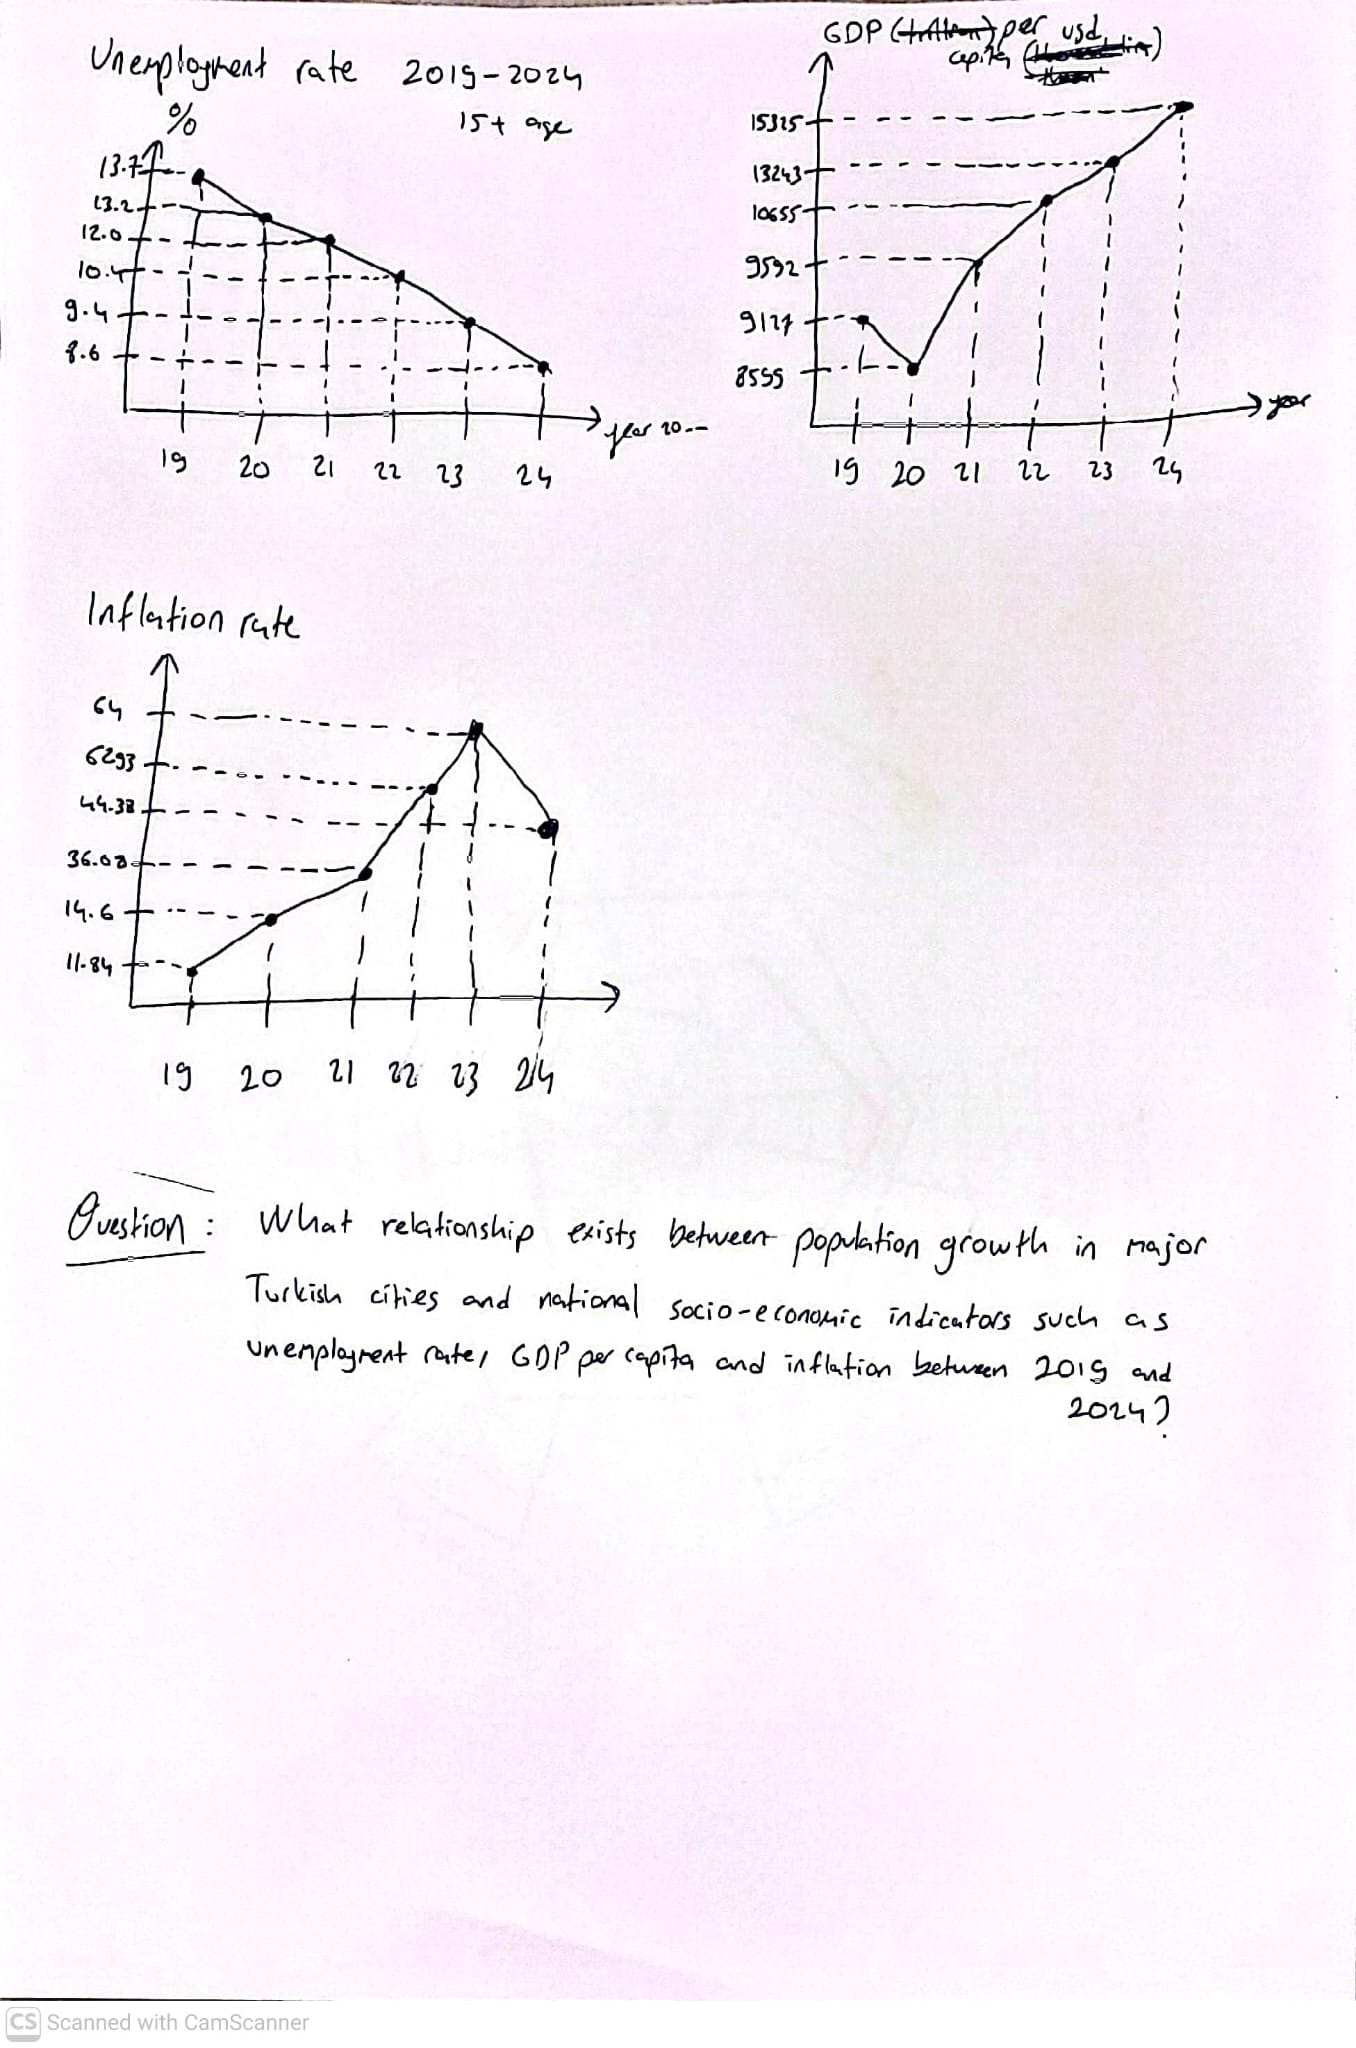
\includegraphics[width=0.58\textwidth,height=0.38\textheight,keepaspectratio]{sketches-images/Task1-B.jpeg}
    \caption{Hand-drawn line charts of unemployment rate, GDP per capita and inflation.}
    \label{fig:task1b-indicators}
\end{figure}

\subsection{Task 1: Formulated Question}

Based on Task 1, the following question was formulated:

\begin{quote}
\textbf{What relationship exists between population growth in major Turkish cities and national socio-economic indicators such as unemployment rate, GDP per capita, and inflation between 2019 and 2024?}
\end{quote}

\textbf{Why this question?}

This question allows us to visually explore possible relationships between urban population and socio-economic indicators such as unemployment, GDP per capita, and inflation

% =========================================================
\section{Task 2: Sketch 1: Multi-Line Comparison View}

\begin{figure}[H]
\centering
\begin{subfigure}{0.47\textwidth}
    \centering
    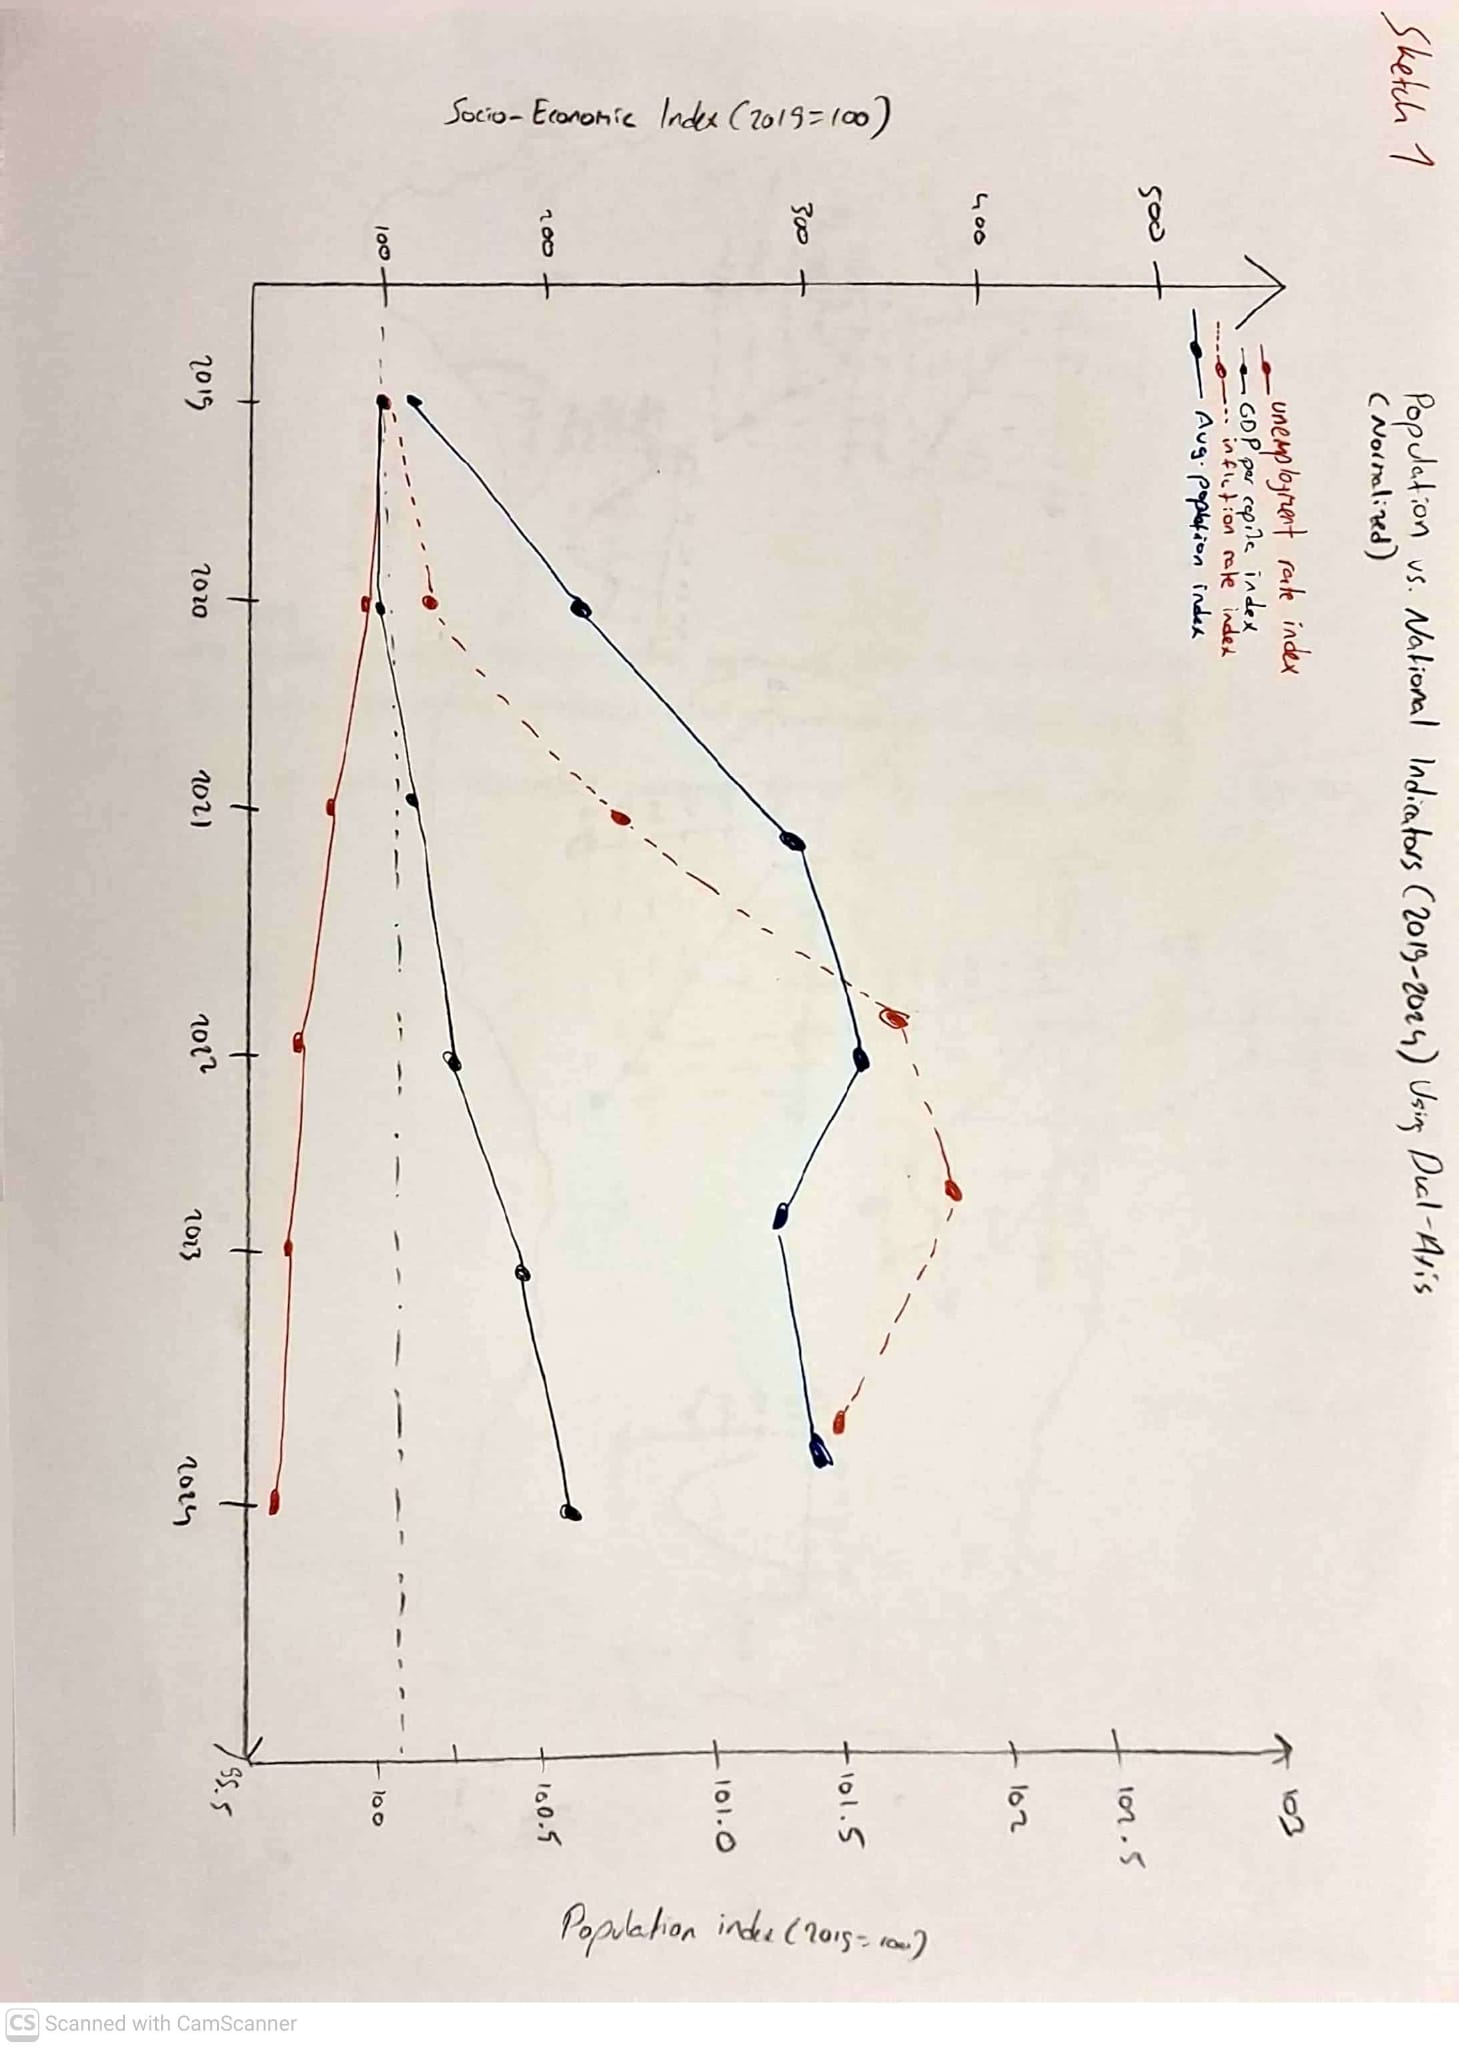
\includegraphics[width=\linewidth,angle=90]{sketches-images/Task2-Sketch1.jpeg}
    \caption{Hand-drawn sketch of the visualization concept.}
\end{subfigure}
\hfill
\begin{subfigure}{0.47\textwidth}
    \centering
    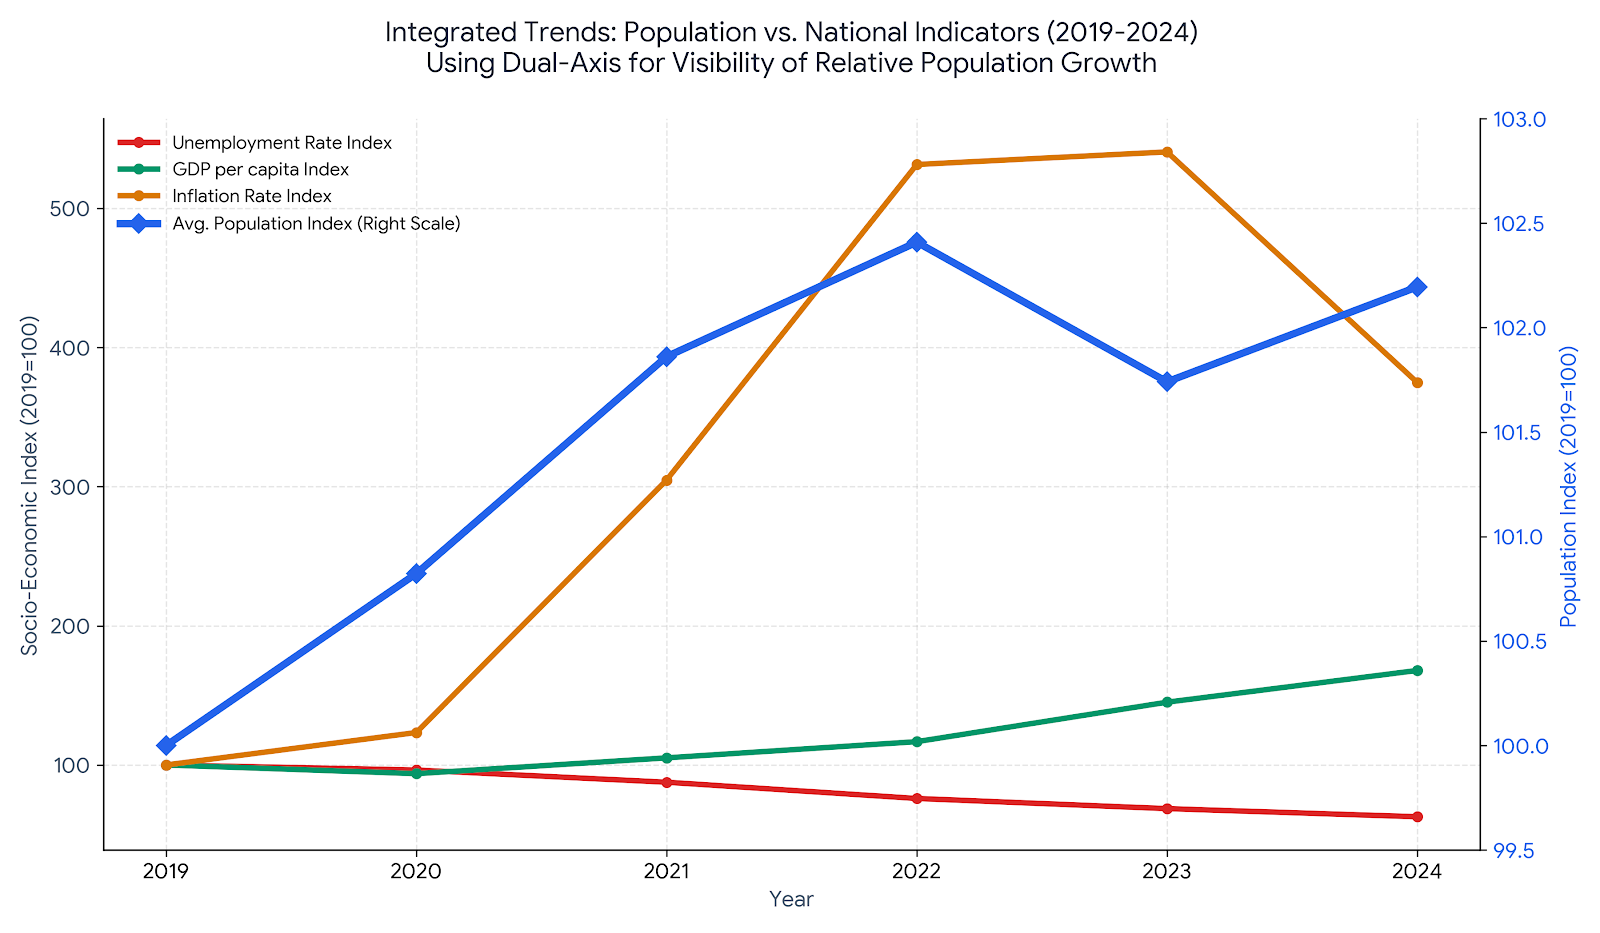
\includegraphics[width=\linewidth]{sketches-images/Sketch1-code-generated.png}
    \caption{Programmatically generated version used to clarify the design.}
\end{subfigure}
\caption{Multi-line comparison visualization showing the relationship between average population growth and national socio-economic indicators between 2019 and 2024.}
\label{fig:sketch1}
\end{figure}

\textbf{Visualization type:} Multi-line comparison chart with dual-axis scaling

\textbf{Goal:}  
The goal of this visualization is to compare temporal trends between population growth in major Turkish cities and national socio-economic indicators such as unemployment rate, GDP per capita, and inflation. By aligning all variables along the same timeline, the visualization helps reveal whether changes in economic conditions coincide with changes in population trends.

\textbf{Design rationale:}

This visualization uses a multi-line chart because it is effective for showing temporal patterns and comparing multiple variables over time. The horizontal axis encodes the time dimension (2019–2024), while vertical position encodes the magnitude of each variable. Different colors represent different indicators, allowing viewers to easily distinguish the trends. Lines and connected points act as visual marks that emphasize direction and slope, making increases or decreases clearly visible. A secondary axis is used for the population index so that variables with different scales can still be compared within the same view. This encoding enables quick identification of correlations, divergences, and turning points between demographic and economic indicators.

\textbf{Where this could be useful:}

This visualization could be useful for policymakers, economists, or researchers interested in understanding how demographic changes in major cities relate to broader economic conditions. It can also support exploratory analysis in educational or analytical settings.

\textbf{Strengths:}
\begin{itemize}[leftmargin=1.5em]
    \item Clearly communicates trends and changes over time.
    \item Enables direct comparison between multiple indicators.
    \item Makes it easier to visually detect possible correlations between variables.
\end{itemize}

\textbf{Weaknesses:}
\begin{itemize}[leftmargin=1.5em]
    \item Dual-axis charts can sometimes be misinterpreted if scales are not carefully labeled.
    \item Too many variables could reduce readability and visual clarity.
\end{itemize}
% -------------------------
\subsection{Sketch 2: Map-Based or Small-Multiple Analytical View}

\begin{figure}[H]
    \centering
    \fbox{\rule{0pt}{2.4in}\rule{0.9\textwidth}{0pt}}
    \caption{Placeholder for Sketch 2 image. Insert the hand-drawn or digital sketch here.}
    \label{fig:sketch2}
\end{figure}

\textbf{Visualization type:} \placeholder{Example: annotated map / small multiples / linked view}

\textbf{Goal:} \placeholder{Explain what this sketch tries to reveal.}

\textbf{Design rationale:}

\placeholder{Explain why this visual form supports geographic context, comparison across cities, or simultaneous reading of multiple variables. Mention visual hierarchy, spatial layout, alignment, direct labeling, or other relevant terms from class.}

\textbf{Where this could be useful:}

\placeholder{Write where or for whom this visualization would be useful.}

\textbf{Strengths:}
\begin{itemize}[leftmargin=1.5em]
    \item \placeholder{Strength 1}
    \item \placeholder{Strength 2}
    \item \placeholder{Strength 3}
\end{itemize}

\textbf{Weaknesses:}
\begin{itemize}[leftmargin=1.5em]
    \item \placeholder{Weakness 1}
    \item \placeholder{Weakness 2}
\end{itemize}

% -------------------------
\subsection{Sketch 3: Abstract Visualization}

\begin{figure}[H]
    \centering
    \fbox{\rule{0pt}{2.4in}\rule{0.9\textwidth}{0pt}}
    \caption{Placeholder for Sketch 3 image. Insert the abstract sketch here.}
    \label{fig:sketch3}
\end{figure}

\textbf{Visualization type:} \placeholder{Example: radial chart / abstract layered composition / symbolic encoding}

\textbf{Goal:} \placeholder{Explain what this sketch tries to reveal.}

\textbf{Design rationale:}

\placeholder{Explain how the abstract design encodes the data, which visual channels it uses, and why abstraction may help show patterns, contrast, rhythm, or relative change. Mention trade-offs between memorability and precision if relevant.}

\textbf{Where this could be useful:}

\placeholder{Write where or for whom this visualization would be useful.}

\textbf{Strengths:}
\begin{itemize}[leftmargin=1.5em]
    \item \placeholder{Strength 1}
    \item \placeholder{Strength 2}
    \item \placeholder{Strength 3}
\end{itemize}

\textbf{Weaknesses:}
\begin{itemize}[leftmargin=1.5em]
    \item \placeholder{Weakness 1}
    \item \placeholder{Weakness 2}
\end{itemize}

% =========================================================
\section{Task 3: Implemented Visualization}

For the implementation stage, one of the three visualization concepts was selected and coded as a standalone HTML file with embedded JavaScript.

\subsection{Chosen Visualization}

\placeholder{Write which sketch you selected and why you selected it for implementation.}

\subsection{Implementation Details}

\begin{itemize}[leftmargin=1.5em]
    \item \textbf{Technology used:} \placeholder{Example: HTML, CSS, JavaScript, D3.js}
    \item \textbf{File structure:} \placeholder{Example: single standalone HTML file}
    \item \textbf{Interaction techniques used:} \placeholder{Example: hover tooltips, highlighting, legends, labels}
    \item \textbf{Visual encoding:} \placeholder{Brief summary of how variables are represented}
\end{itemize}

\subsection{GitHub Repository}

The implementation can be found at the following link:

\githublink

Replace the placeholder link above with your actual repository link.

\subsection{Screenshots of the Final Visualization}

\begin{figure}[H]
    \centering
    \fbox{\rule{0pt}{2.5in}\rule{0.9\textwidth}{0pt}}
    \caption{Placeholder for screenshot of the implemented visualization.}
    \label{fig:implementation1}
\end{figure}

\begin{figure}[H]
    \centering
    \fbox{\rule{0pt}{2.5in}\rule{0.9\textwidth}{0pt}}
    \caption{Placeholder for an additional screenshot, such as interaction state, tooltip, or focused view.}
    \label{fig:implementation2}
\end{figure}

\subsection{Implementation Reflection}

\placeholder{Write a short reflection about whether the coded version successfully answered the research question, what worked well, and what could still be improved.}

% =========================================================
\section{Discussion}

\placeholder{In this section, summarize the main visual patterns you observed after sketching and implementation. For example, mention whether some cities show steady growth while others fluctuate, and whether those changes appear to move together with unemployment, GDP per capita, or inflation. Keep this section interpretive rather than purely descriptive.}

% =========================================================
\section{Conclusion}

This homework explored the relationship between urban population change and national socio-economic indicators in Türkiye between 2019 and 2024. The project involved three stages: exploratory sketching, concept generation, and coded implementation. Through these stages, the report aimed to move from raw tabular values toward visual forms that support comparison, trend analysis, and interpretation.

\placeholder{Add 1 short paragraph here summarizing your final takeaway.}

% =========================================================
\section*{Appendix A: Optional Source Image Placeholder}

If you want to include the source screenshot that contains the socio-economic indicator values, you may place it here.

\begin{figure}[H]
    \centering
    \fbox{\rule{0pt}{2.7in}\rule{0.9\textwidth}{0pt}}
    \caption{Placeholder for the source image containing unemployment, GDP per capita, and inflation values.}
    \label{fig:source-image}
\end{figure}

\textit{Optional note:} If the image file is stored locally, replace the placeholder above with a command such as:

\begin{verbatim}
\includegraphics[width=0.85\textwidth]{tuik_indicators.png}
\end{verbatim}

% =========================================================
\section*{Appendix B: Practical Notes for Replacing Placeholders}

\begin{itemize}[leftmargin=1.5em]
    \item To replace an image placeholder, use:
\begin{verbatim}
\includegraphics[width=0.9\textwidth]{your-image-file-name}
\end{verbatim}
    \item For large hand-drawn sketches, using \verb|[width=0.8\textwidth]| or \verb|[width=0.9\textwidth]| usually works well.
    \item If you want to place two screenshots side by side, use the \verb|subfigure| environment from the \verb|subcaption| package.
    \item If your GitHub repository contains a single HTML file, mention that it can be opened directly in a browser.
\end{itemize}

\end{document}
